\item O cilindro de \SI{50}{\kilogram} tem uma velocidade angular de \SI{30}{\radian/\second} quando é colocado em contato com a superfície em $C$. Se o coeficiente de atrito cinético é $\mu_{k}=0.2$, determine quanto tempo vai levar para o cilindro parar de girar. Que força é desenvolvida no membro $AB$ durante esse tempo? O eixo através do cilindro está conectado a dois membros simétricos (apenas $AB$ é mostrado). Para o cálculo, despreze o peso dos membros.

\import{../answers}{answer-3}

\vspace{-1.2cm}
\begin{flushright}
	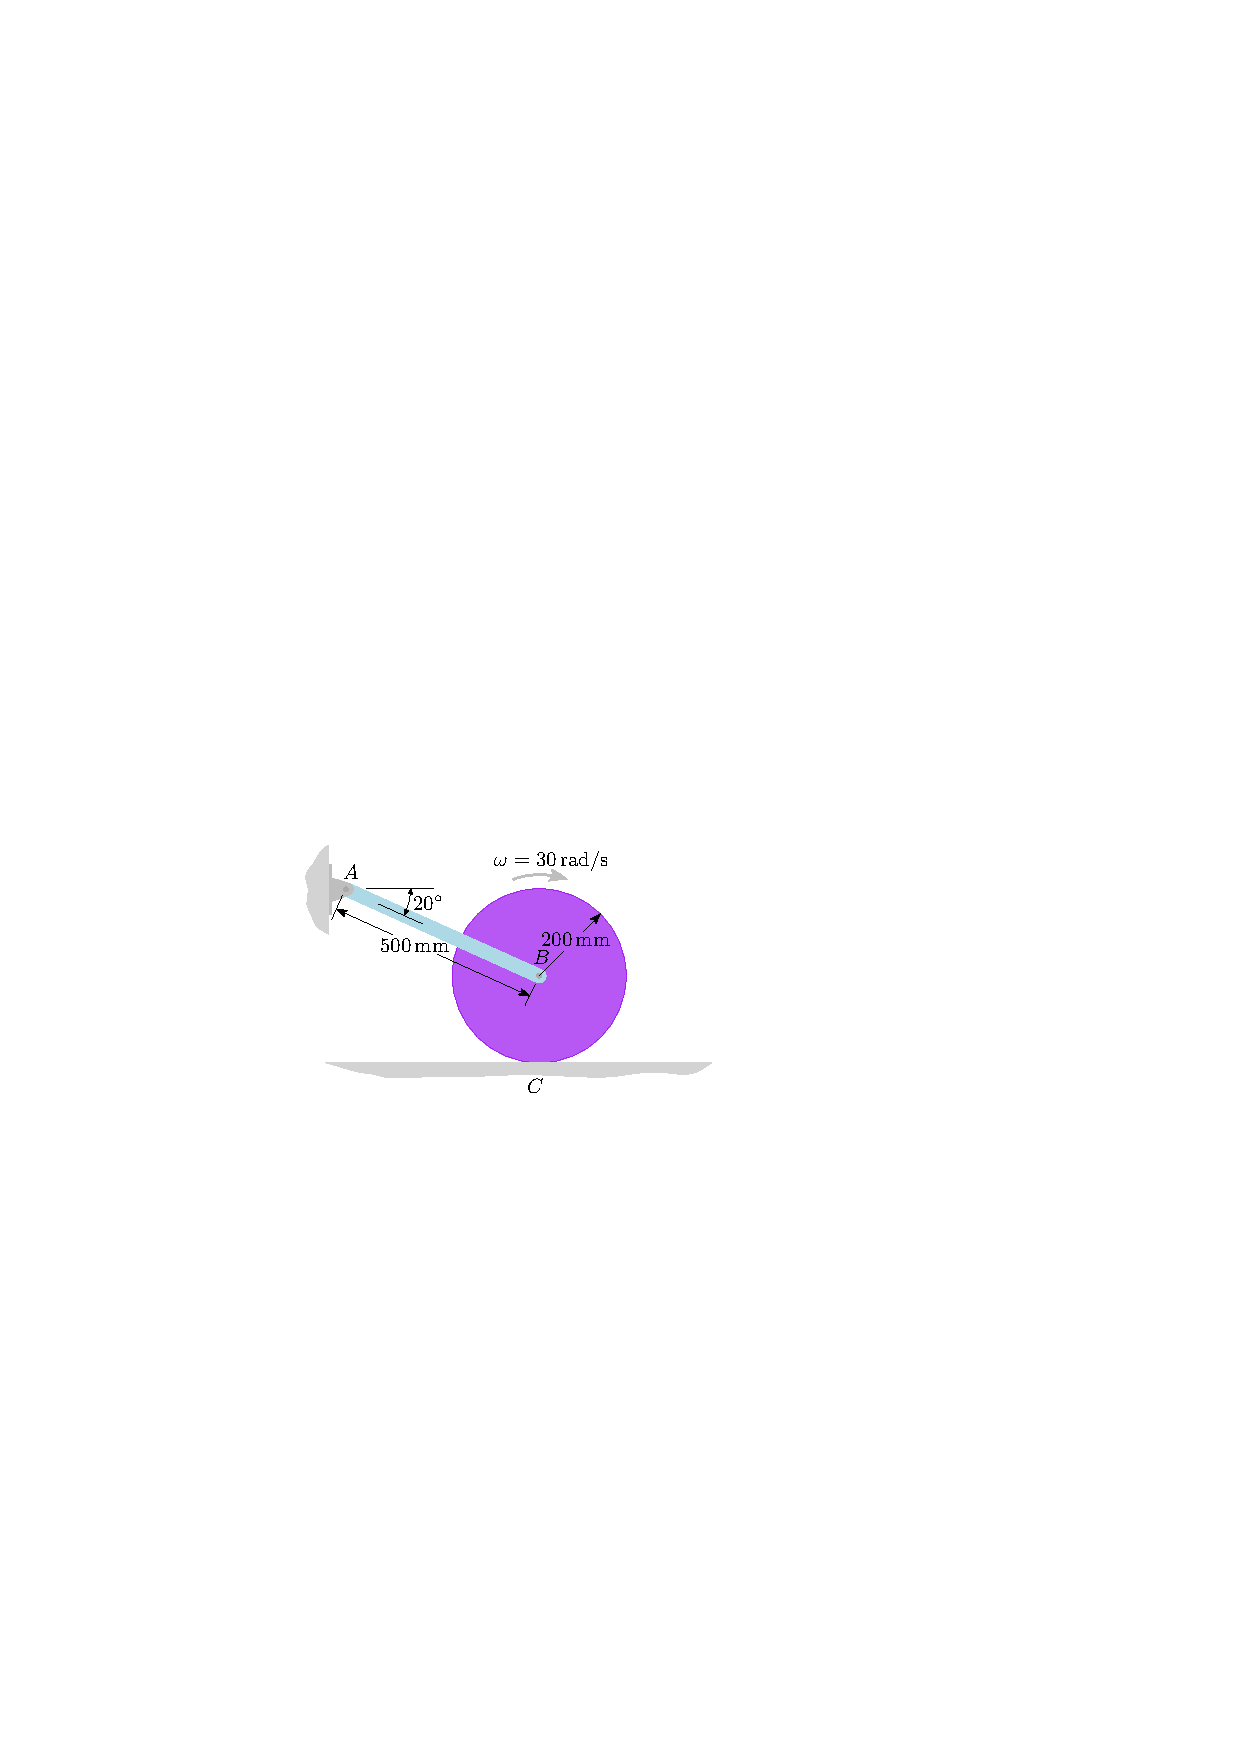
\includegraphics[scale=1.3]{../../images/draw_1_1}
\end{flushright}  